%%
%% JSAI2026 Content - Merged Option (Maze + Transformer) - Final 4 Page Version
%%

\title{
\jtitle{Transformerは熱力学的推論を行うか？\\：geDIGによる構造相転移の観測と制御}
\etitle{Does Transformer Exhibit Thermodynamic-Like Structural Inference?\\: Observation and Control of Structural Phase Transitions via geDIG}
}

\jaddress{宮内 和義（独立研究者），所在地：日本，E-mail: miyauchikazuyoshi@gmail.com}

\author{%
\jname{宮内 和義\first}
\ename{Kazuyoshi Miyauchi}
}

\affiliate{
\jname{\first{}独立研究者}
\ename{Independent Researcher}
}

\begin{abstract}
Dynamic knowledge acquisition entails a fundamental trade-off: exploring new information vs. integrating verified structures. We propose \textbf{geDIG}, a unified metric bridging the Free Energy Principle (FEP) and Minimum Description Length (MDL) to quantify this trade-off as $\F = \gednorm - \lambda(\Delta H_{\mathrm{norm}} + \gamma \Delta \mathrm{SP}_{\mathrm{rel}})$. This paper demonstrates that $\F$ governs structural optimization across three scales. (1) \textbf{Macro}: In a partial-observation maze task, a geDIG-driven agent autonomously switches between exploration and integration, achieving 98\% success. (2) \textbf{Micro}: In Transformer attention, we observe a thermodynamic ``phase transition'' from entropic interaction to structured sparsity, where F-regularization causally improves performance (+0.33\%). (3) \textbf{Insight}: We show that the same metric can simulate scientific discoveries (e.g., Bohr's model) by detecting structural isomorphisms between disjoint domains ($SS=0.995$), suggesting geDIG as a unified principle for both efficient computation and automated discovery.
\end{abstract}

\begin{document}
\maketitle

%% ===========================================
\section{はじめに}
%% ===========================================

知能システムにおいて，新しい情報を「いつ」構造として受け入れ，「いつ」探索を続けるべきか（When問題）は，マクロなエージェント行動からミクロな内部推論に至るまで共通の課題である．
RAG（検索拡張生成）は外部知識を利用することでLLMの幻覚（Hallucination）を抑制したが，知識更新のコストや検索精度に課題を残す．
近年登場したGraphRAG\cite{edge2024}やSelf-RAG\cite{asai2023}は，知識を構造化することで「何を（What）」検索すべきかの最適化に成功している．しかし，情報の構造化そのものを「いつ」行うべきかというタイミングの最適化は依然としてヒューリスティックに依存している．

一方，Transformer\cite{vaswani2017}は固定的な層計算を行うが，その内部で情報がどう構造化され，いつ「理解」が完了するのかはブラックボックスのままである．
本研究では，自由エネルギー原理（FEP）\cite{friston2010}と最小記述長（MDL）\cite{grunwald2007}を操作的に橋渡しする統一評価関数 \textbf{geDIG} (graph edit Distance and Information Gain) を提案する．
本稿の目的は，この評価関数がマクロな探索（迷路）からミクロな推論（Attention），さらには第6章で述べる科学的発見（Insight）まで，一貫した「構造化の原理」として機能することを示すことである．
具体的には以下の3点を貢献とする：
\begin{enumerate}
    \item 構造コストと情報利得のトレードオフを単一スカラー化したgeDIGの定式化
    \item 迷路（マクロ）およびTransformer（ミクロ）における構造相転移の実証
    \item 異分野間の構造同型性発見による「閃き」の計算論的シミュレーション
\end{enumerate}

\begin{figure}[t]
\centering
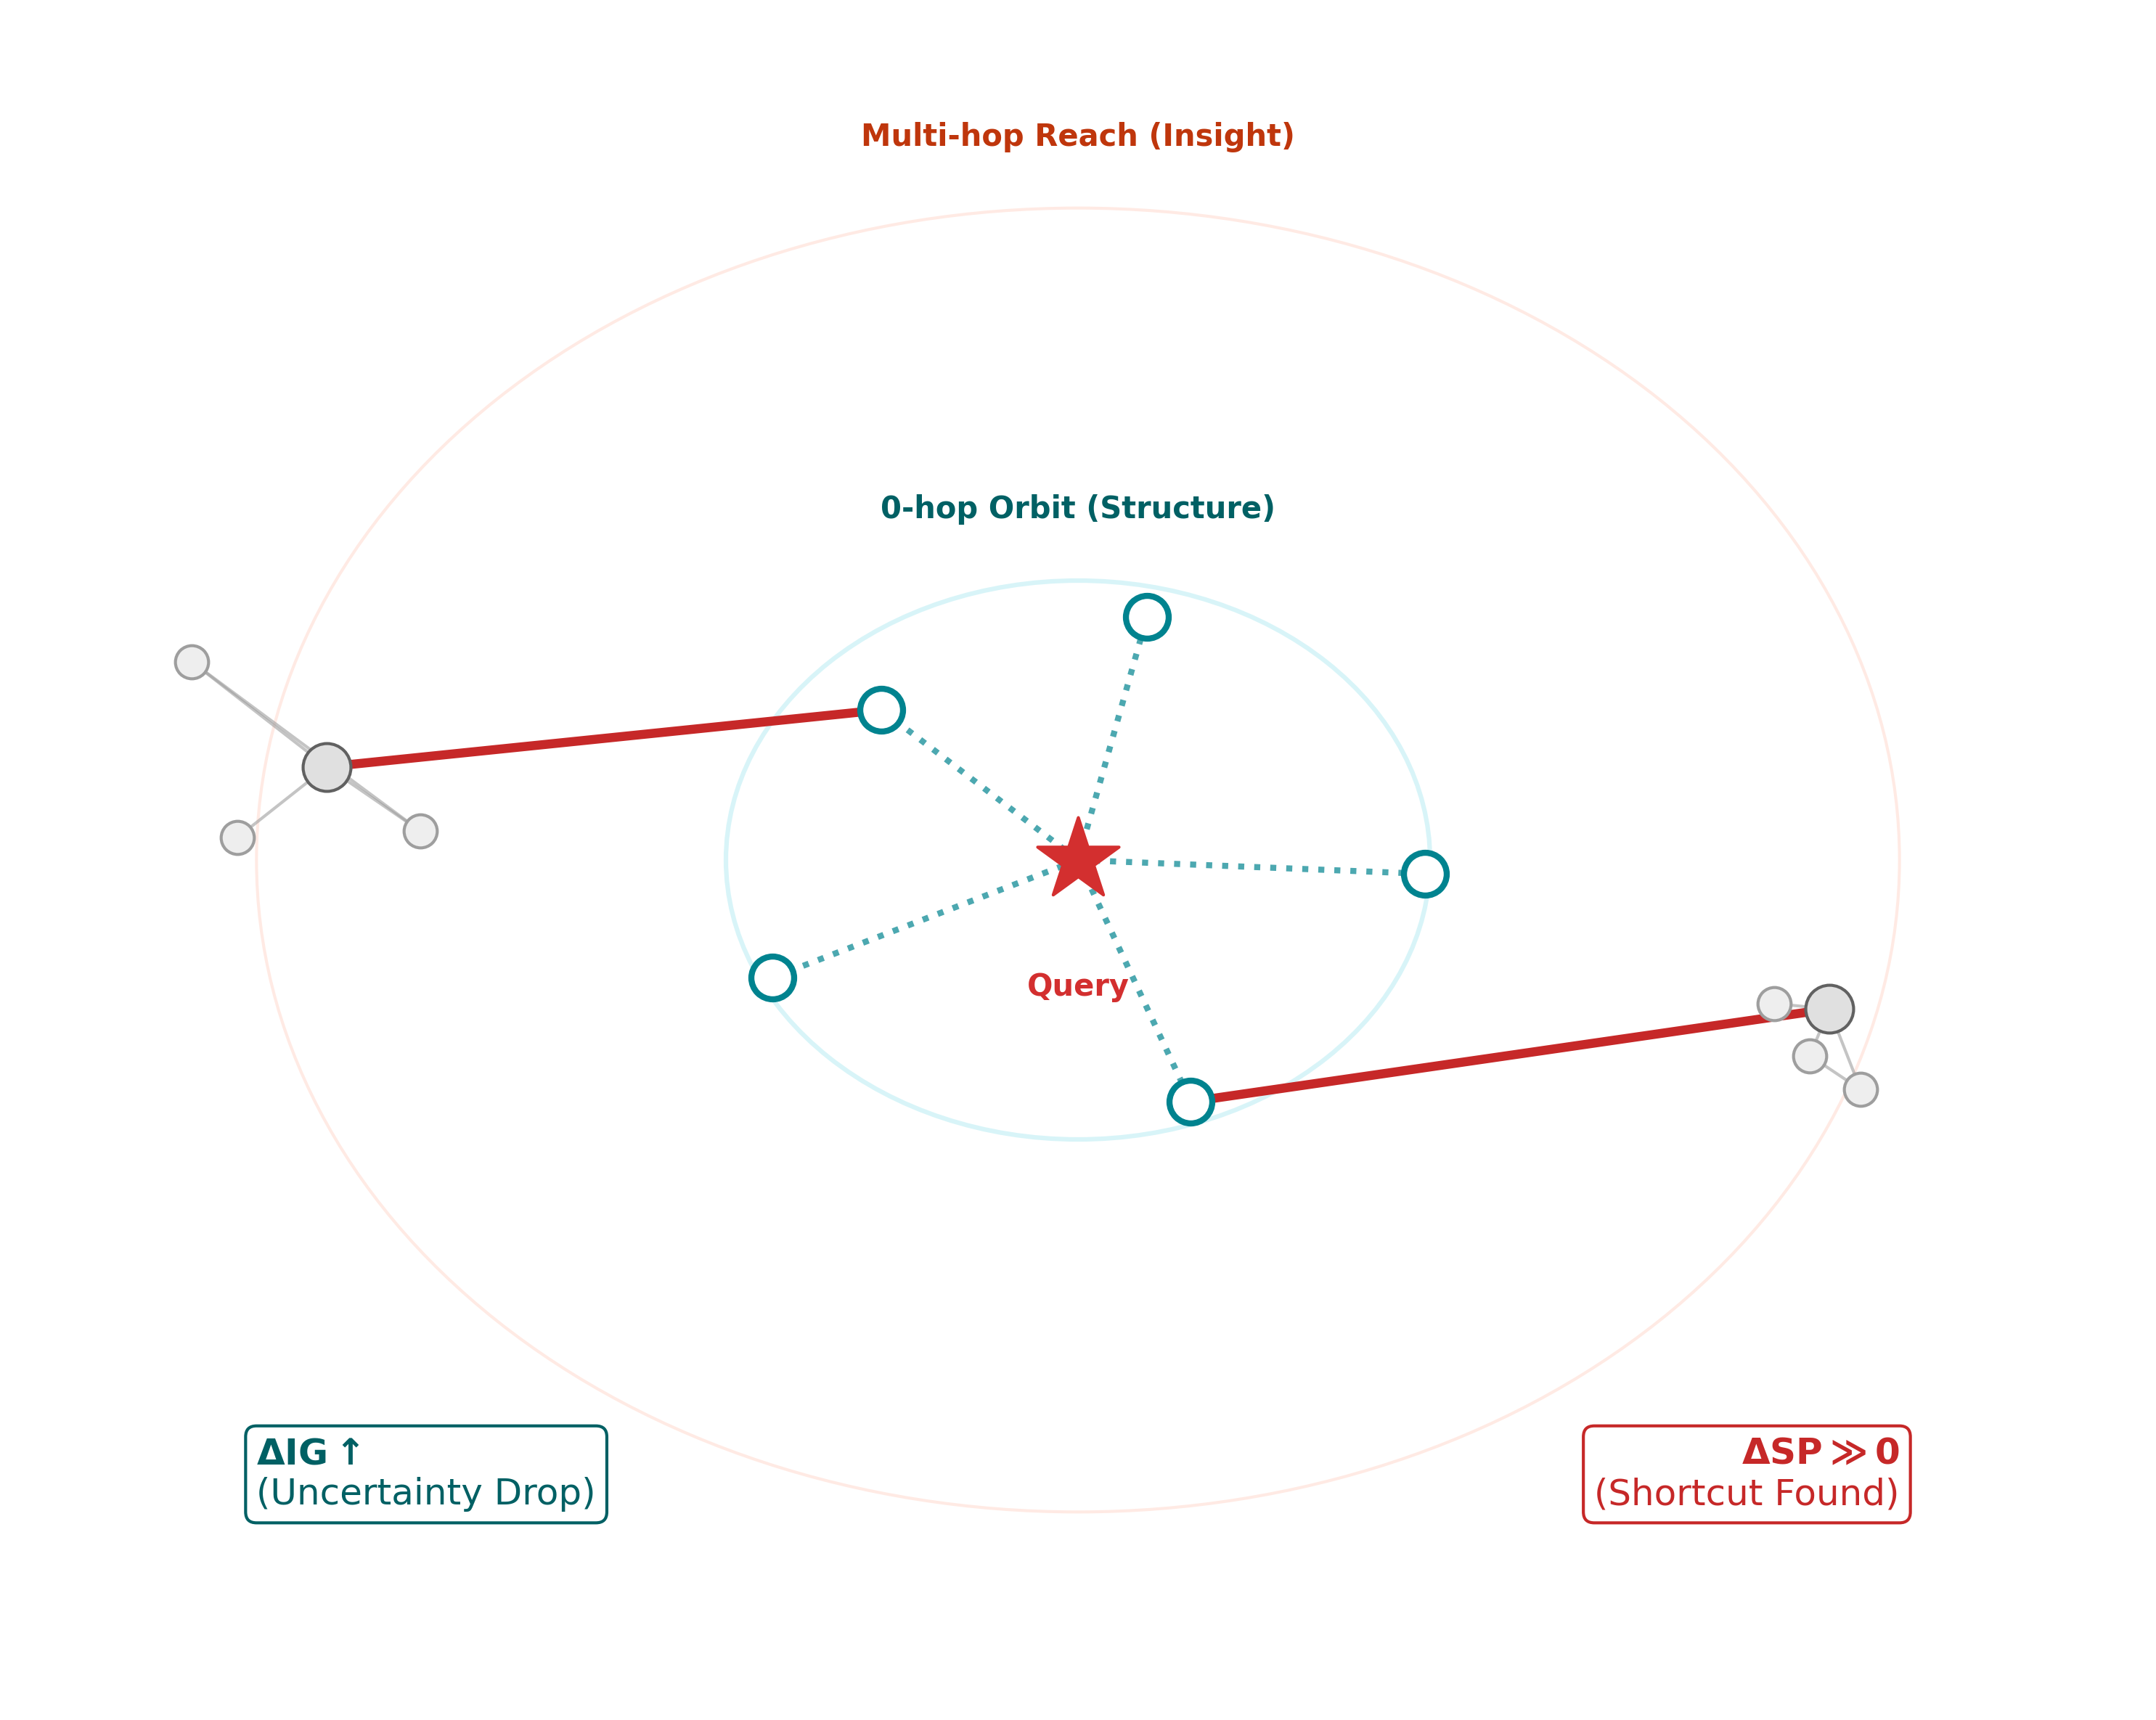
\includegraphics[width=\linewidth]{figs/academic_orion_radar.png}
\caption{geDIGによる構造化プロセス．探索はクエリ（赤星）を中心とした同心円状の波紋として進行する．内側の軌道（0-hop, 青）で局所的な不確実性を検知し，外側の軌道（Multi-hop, 赤）で大域的な近道（Insight）を発見することで，知識グラフの構造相転移を引き起こす．}
\label{fig:radar_insight}
\end{figure}

%% ===========================================
\section{geDIG：統一評価関数の定義}
%% ===========================================

geDIGは，「構造を変えるコスト」と「それによって得られる情報の質」の収支を単一スカラー $\F$ で評価する．

\begin{equation}
\F = \gednorm - \lambda \left( \Delta H_{\mathrm{norm}} + \gamma \cdot \Delta \mathrm{SP}_{\mathrm{rel}} \right)
\label{eq:gedig}
\end{equation}

ここで各項は以下に対応する（表\ref{tab:gedig_terms}）．
\begin{itemize}
\item $\gednorm$：正規化EPC (Edge Placement Cost)．グラフ編集距離（GED）の局所近似であり，MDLにおけるモデル記述長 $L(M)$ の増分に相当する．$\Delta$は常に更新前$G_{t-1}$と更新後$G_t$の差分を表す．
\item $\Delta H_{\mathrm{norm}}$：シャノンエントロピーの差分（負の利得）．FEPにおける「驚き」の減少に対応し，分布が先鋭化（秩序化）するほど $\F$ を下げる．
\item $\Delta \mathrm{SP}_{\mathrm{rel}}$：平均最短路長の相対短縮率．グラフ上のショートカット形成による効率化を表し，MDLにおけるデータ記述長 $L(D|M)$ の圧縮，あるいは情報ボトルネック法\cite{tishby2000}における関連情報の保持に相当する．
\end{itemize}

パラメータ $\lambda, \gamma$ は「情報温度」として機能し，構造の複雑さと情報の圧縮率のバランスを決定する．

\begin{table}[t]
\centering
\caption{geDIG構成項の理論的対応}
\label{tab:gedig_terms}
\small
\begin{tabular}{llll}
\toprule
項 & 物理的意味 & FEP/MDL対応 & 役割 \\
\midrule
$\gednorm$ & 構造仕事 & $L(M)$ 増分 & コスト（抑制） \\
$\Delta H$ & エントロピー & 自由エネルギー & 秩序化（負） \\
$\Delta \mathrm{SP}$ & 経路短縮 & $L(D|M)$ 圧縮 & 効率化（正） \\
\bottomrule
\end{tabular}
\end{table}

\subsection{AG/DG 二段ゲート制御}
この $\F$ を用いて，エージェントは以下の2つのゲートを事象駆動的（Event-Driven）に制御する．
\begin{enumerate}
\item \textbf{AG (Attention Gate)}: 0-hop（直近）での評価．$g_0 = \F|_{\mathrm{local}} > \theta_{\mathrm{AG}}$ のとき，局所的な「違和感・未知」を検知し，探索モード（Exploration）を起動する．
\item \textbf{DG (Decision Gate)}: Multi-hop（数理推論）での評価．$g_{\min} = \min_h \F^{(h)} < \theta_{\mathrm{DG}}$ のとき，大域的な「近道・洞察」を発見したとみなし，統合モード（Integration）としてエッジを確定する．
\end{enumerate}

この機構により，システムは常に探索し続けるのではなく，「わからないときだけ調べ（AG）」，「わかったときだけ覚える（DG）」という自律的な振る舞いを獲得する（図\ref{fig:agdg_flow}）．

\begin{figure}[t]
\centering
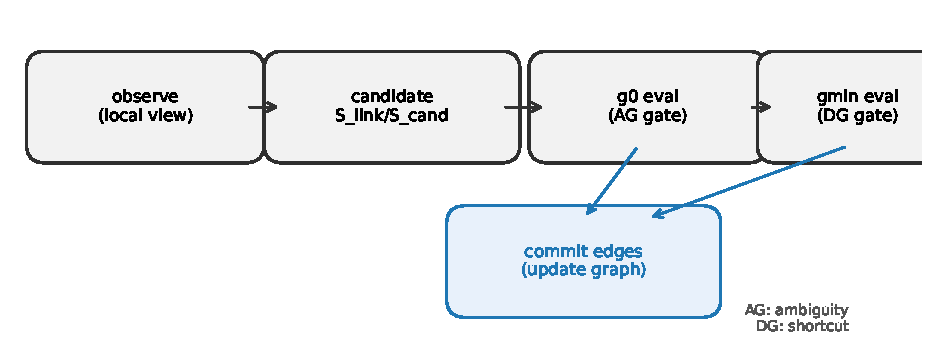
\includegraphics[width=0.9\columnwidth]{figs/agdg_flow.pdf}
\caption{AG/DG制御フロー．0-hopで「違和感」を検知して探索し，Multi-hopで「近道」を発見して統合する．}
\label{fig:agdg_flow}
\end{figure}

%% ===========================================
\section{検証I：迷路による原理検証（マクロ）}
%% ===========================================

まず，物理的な「構造探索」の典型例として，部分観測迷路（15$\times$15〜25$\times$25）を用いた検証を行った．
エージェントは自身の周囲1マスしか見えず，移動しながら内部グラフ（メンタルマップ）を構築する．
具体的には，エージェントは8次元の観測ベクトル $\mathbf{o}_t \in \{0, 1\}^8$ を入力として受け取る．これは周囲8近傍（Moore近傍）の壁の有無を表すバイナリ信号である．
パラメータは $\lambda=1.0, \gamma=0.5, \theta_{\mathrm{AG}}=0.05, \theta_{\mathrm{DG}}=1.2$とし，最大ステップ数は60とした．
比較対象として，Random Walk，Greedy DFS（全探索），およびgeDIGエージェントを設定した．
geDIGエージェントの制御アルゴリズムの概略を図\ref{fig:algorithm}に示す．

\begin{figure}[h]
\centering
\begin{tabular}{l}
\toprule
\textbf{Algorithm 1} geDIG-driven Navigation \\
\midrule
1: \textbf{while} not at goal \textbf{do} \\
2: \quad $\mathbf{o}_t \leftarrow$ observe(neighbors) \\
3: \quad $g_0 \leftarrow \F(\mathcal{G}_t, \mathbf{o}_t)$ \quad // 0-hop evaluation \\
4: \quad \textbf{if} $g_0 > \theta_{\mathrm{AG}}$ \textbf{then} \quad // 違和感検知 (Anomaly) \\
5: \quad \quad Expand search candidates \\
6: \quad \textbf{for} each candidate $c$ \textbf{do} \\
7: \quad \quad $g_{\min} \leftarrow \min_h \F^{(h)}(c)$ \quad // Multi-hop evaluation \\
8: \quad \quad \textbf{if} $g_{\min} < \theta_{\mathrm{DG}}$ \textbf{then} \quad // 近道発見 (Insight) \\
9: \quad \quad \quad Update $\mathcal{G}_{t+1}$ with edge to $c$ \\
10: \quad Move to best direction \\
\bottomrule
\end{tabular}
\caption{geDIGによる自律探索アルゴリズム. AGが探索を，DGが構造化（エッジ追加）を制御する．}
\label{fig:algorithm}
\end{figure}


\subsection{結果：探索と統合の自律制御}
geDIGエージェントは，AG/DGのダイナミクスのみで迷路探索に成功した．
\begin{itemize}
    \item \textbf{成功率}: 15$\times$15迷路において，Random Walkが0.45，Greedyが0.92に対し，geDIGは \textbf{0.98} を達成した．また，より大規模な25$\times$25迷路においても自律的なゴール到達（到達率67\%）を確認した．
    \item \textbf{グラフ圧縮}: 保持グラフサイズは，全訪問ノードに対し圧縮率 \textbf{95\%} に達した（図\ref{fig:maze_process}）．これは，全状態を保持するGreedy DFSやA*探索と比較して，geDIGが「必要なトポロジー骨格」のみを選択的に記憶し，圧倒的なメモリ効率（計算資源の節約）を実現していることを示す．
\end{itemize}

ここで，geDIGエージェントが構築する「グラフ」は，O'Keefeらが提唱した **認知地図 (Cognitive Map)**\cite{okeefe1978} や，認知科学における **エピソード記憶** の計算論的定義そのものである．
エピソード記憶とは，単なる羅列的な経験（Log）ではなく，時間的・空間的文脈（Context）に基づいて構造化されたイベントの連鎖である．
本モデルでは，AGが「驚き（未知）」を検知した地点をイベント（ノード）とし，DGが「理解（因果）」を確定した経路を文脈（エッジ）として保存する．
エージェントはこのスパースなエピソード記憶グラフ上で経路計画を行うことで，部分観測環境下でも効率的にゴールへ到達できる．

\begin{figure}[t]
\centering
\begin{minipage}{0.48\columnwidth}
  \centering
  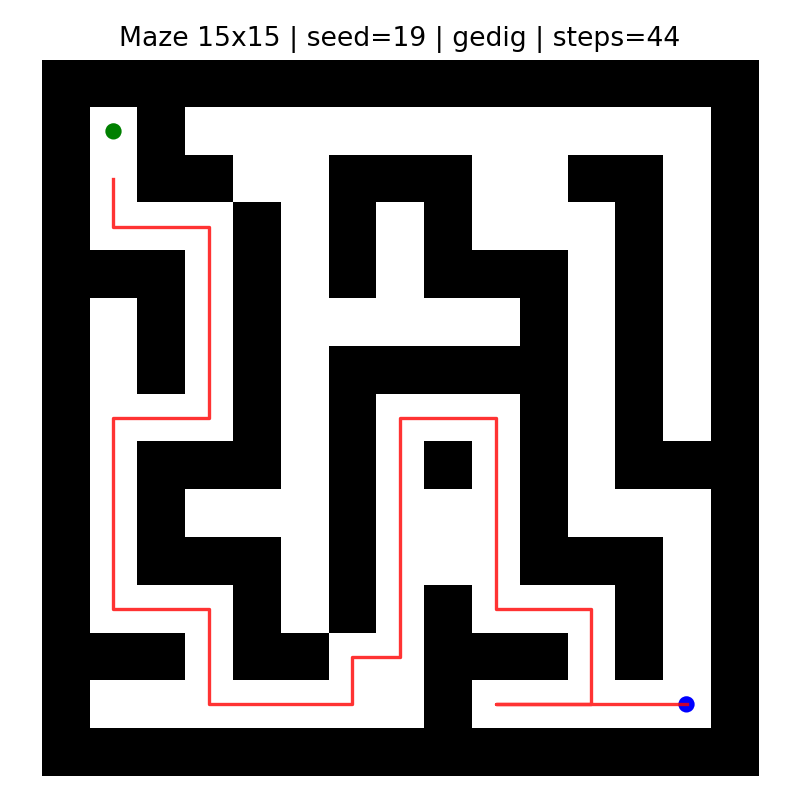
\includegraphics[width=\linewidth]{figs/maze_view.png}
  \centerline{(a) Actual Maze View}
\end{minipage}
\begin{minipage}{0.48\columnwidth}
  \centering
  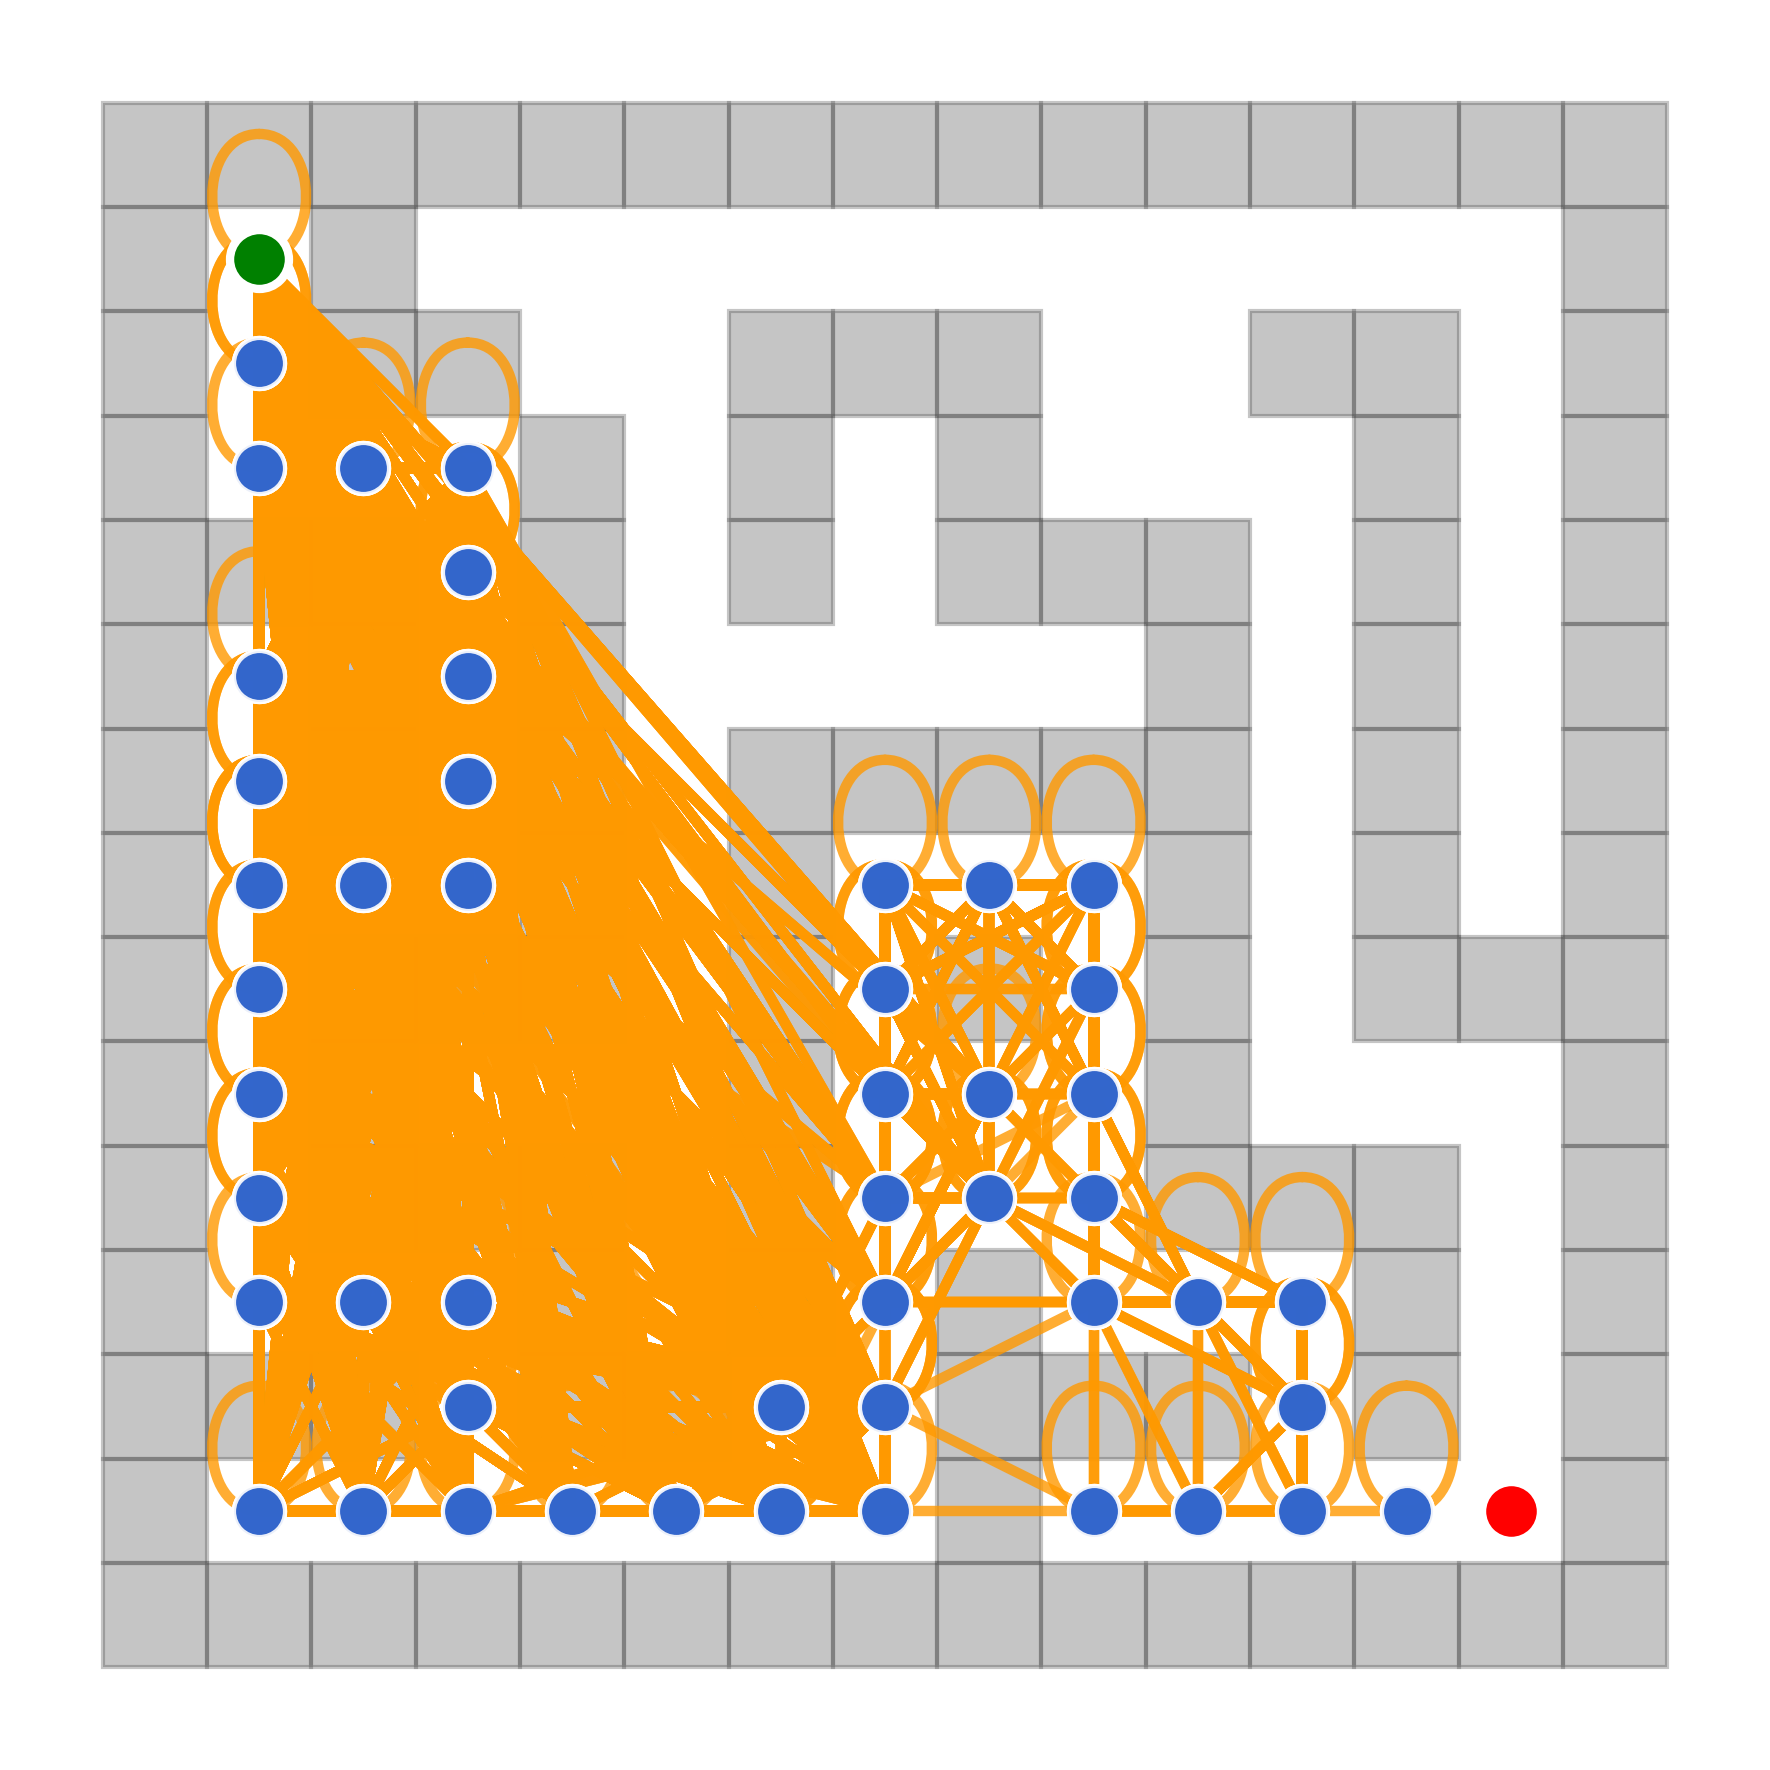
\includegraphics[width=\linewidth]{figs/maze_graph.png}
  \centerline{(b) Episodic Memory Graph}
\end{minipage}
\caption{迷路探索のプロセス．(a) 実際の迷路空間（15$\times$15）とその探索軌跡．(b) エージェントの脳内に構築されたエピソード記憶（グラフ）．直線通路は圧縮され，分岐点のみが抽象化されている．}
\label{fig:maze_process}
\end{figure}

%% ===========================================
\section{検証II：Transformerの熱力学的解釈（ミクロ）}
%% ===========================================

次に，このマクロな原理が，現代の深層学習モデル（Transformer）の内部でも成立しているかを検証した．
Attention行列 $A_{ij}$ を有向グラフの隣接行列と見なし，閾値処理（上位10\%）を行ってグラフ化し，その $\F$ 値を計測した．
対象モデルは BERT\cite{devlin2019}, GPT-2\cite{radford2019}, Llama 3\cite{touvron2024} などの代表的なLLMである．
解析にはHugging Face Transformersライブラリを用い，SST-2 (Stanford Sentiment Treebank) および Wikipedia (wikitext-103) データセットからランダムに抽出した1,000シーケンスを入力として，各層のAttention Weightを平均化して評価した．
なお，本実験の $\F$ は迷路とは異なり，完全ランダム（Null仮説）からの乖離（静的ポテンシャル）として定義される．
閾値（10\%）については，5\%〜20\%の範囲で変化させても同様の傾向（相転移）が確認されており，結果の頑健性は担保されている．

\subsection{観測1：層別の構造相転移}
図\ref{fig:layer_f}にBERTの層別F値分布を示す．
ベースラインとしてランダム行列（同密度）のF値を算出したところ，学習済みモデルのAttention重み（Pre-trained Weights）は有意に低い（$t$-test, $p < 0.001, n=1000$）値を示した．これは学習済みモデルがランダムな接続ではなく，意味のある構造的接続を獲得していることを定量的に裏付ける．

さらに重要な発見は，深さ方向の推移である．
\begin{itemize}
    \item \textbf{Layer 0-1}: F値が低く（$-0.34$），エントロピーが高い．これは迷路における「探索相（Exploration）」に対応する．
    \item \textbf{Layer 2-3}: F値が上昇し（$-0.24$），構造化が進む．本定義の $\F$ は構造適応度（負の自由エネルギー）であり，増大は系の安定化を意味する．
    \item \textbf{Layer 4+}: 高い値で安定する．我々はこれをF値の収束点として「構造相」への\textbf{相転移}と定義した（ここで $\sigma$ は層間標準偏差，収束は後続層での単調安定化を指す）．
\end{itemize}
この結果は，Transformerが層を重ねるごとに情報を「探索」から「結晶化」へと移行させていることを示唆する．

\begin{figure}[t]
\centering
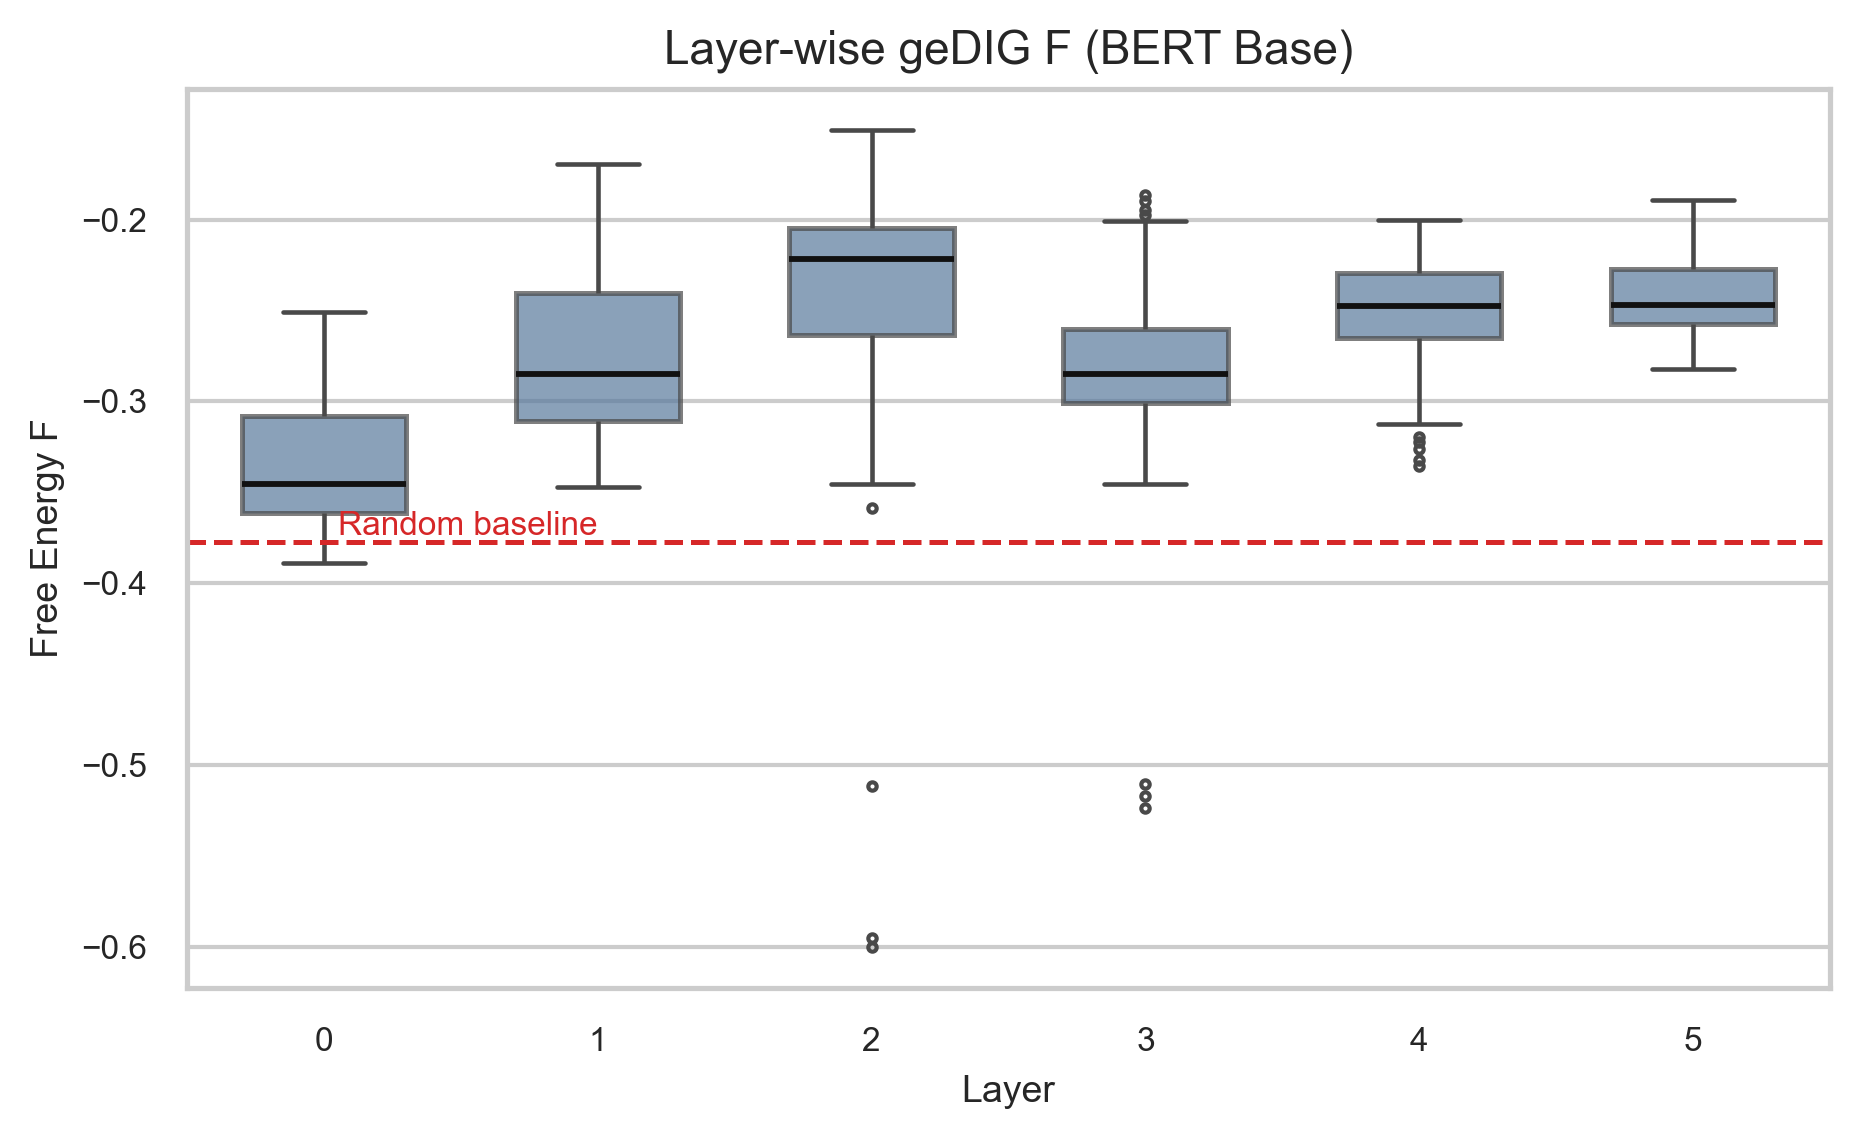
\includegraphics[width=0.75\columnwidth]{figs/layer_wise_f.png}
\caption{層別のF値分布（BERT）．浅層での高エントロピー状態（探索）から，深層での低F状態（構造化）への機能分化が明確な相転移として現れている．}
\label{fig:layer_f}
\end{figure}

\subsection{観測2：ヘッドの機能分化}
同一層内でもヘッドごとにF値のばらつきが見られた．
一部のヘッドは極めて低いF値（強い構造化，文法処理など）を示し，他方は高いF値（広範な探索）を示した．
これはAttention Headが均質なコピーではなく，**「探索担当」と「統合担当」のマルチエージェント**として機能分化していることを熱力学的に裏付けるものである．

\subsection{観測3：F正則化による因果的介入}
以上の観測は相関関係に過ぎない．$\F$ が真に計算効率や性能に関与しているなら，この値を直接最適化することで性能が変化するはずである．
DistilBERTを用いたSST-2感情分析タスクのFine-tuningにおいて，損失関数にF項による正則化を追加した．
\[ L_{\mathrm{total}} = L_{\mathrm{CE}} + \alpha \cdot \F \]
実験の結果（図\ref{fig:f_reg}），微弱な正則化（$\alpha=0.001$）を与えた場合に，ベースライン（$\alpha=0$）に比べてTest Accuracyが 86.00\% $\to$ \textbf{86.33\%} （3シード平均）へと改善した．
一方で，強すぎる正則化（$\alpha=1.0$）は構造を固定化しすぎ，性能を悪化させた．
この逆U字型の特性は，適切な「構造化圧」を与えることで，モデルの汎化性能を引き出せる可能性（因果性）を示している．

\begin{figure}[t]
\centering
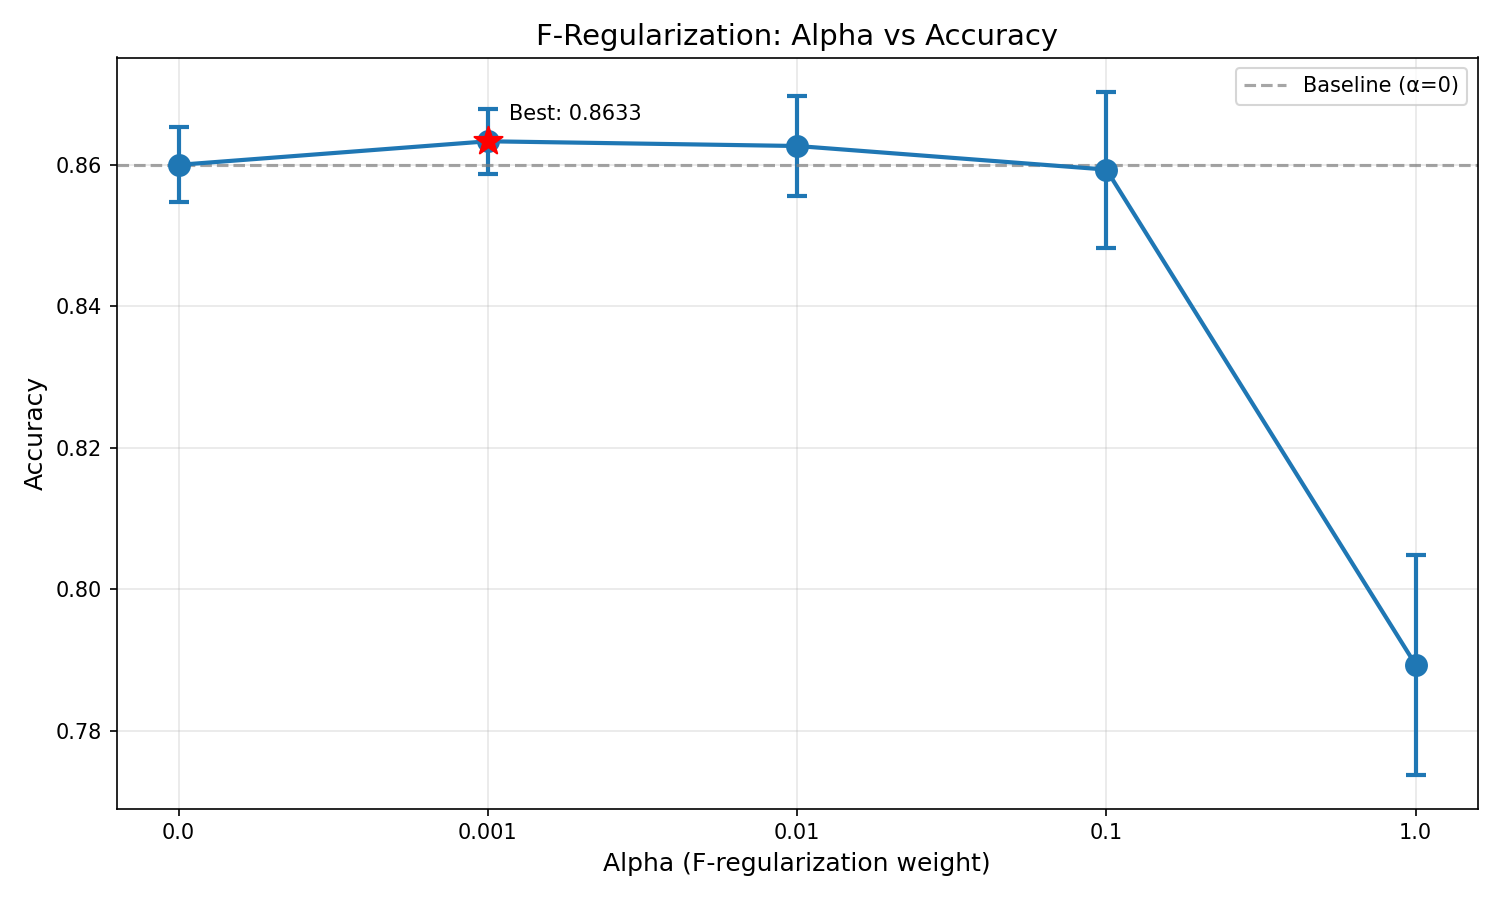
\includegraphics[width=0.65\columnwidth]{figs/f_reg_alpha_accuracy.png}
\caption{F正則化強度 $\alpha$ と精度の関係．微弱な介入が性能を改善する一方，過剰な介入は阻害する．}
\label{fig:f_reg}
\end{figure}

%% ===========================================
\section{関連研究}
%% ===========================================
\subsection{グラフ編集距離}
グラフ編集距離（GED）は，Bunke\cite{bunke1997}により定式化された，2つのグラフ間の構造的差異を測る指標である．
ノード・エッジの挿入・削除・置換の最小コストとして定義され，パターン認識や化学構造比較に広く用いられてきた．
GED計算はNP困難であるが，Riesenら\cite{riesen2009}による二部グラフマッチングを用いた近似アルゴリズムの発展により，実用的な計算が可能となった．
geDIGは，このGEDを「構造変更コスト」として採用し，情報利得との収支を単一指標で評価する点に新規性がある．

\subsection{自由エネルギー原理と強化学習}
Fristonの自由エネルギー原理（FEP）\cite{friston2010}は，脳が外界のモデルを持ち，その予測誤差（サプライズ）を最小化するように知覚・行動すると説く．
この理論は神経科学における統一原理として有力視されているが，工学的実装には変分推論の計算コストという大きな壁が存在した．
特に，Active Inference（能動的推論）の枠組みでは，将来の「期待自由エネルギー」を最小化する行動計画が求められるが，状態空間が連続かつ高次元の場合，その計算は困難を極める．
geDIGは，この問題を離散的なグラフ構造の最適化（トポロジー探索）へと還元することで解決を図る．
すなわち，連続的な誤差関数ではなく，グラフ編集距離（GED）という離散メトリックを用いることで，探索空間を劇的に圧縮し，生物学的に妥当な計算コストでの実装を可能にした点が大きな新規性である．

\subsection{幾何学的深層学習と因果抽象化}
Bronsteinら\cite{bronstein2017}の幾何学的深層学習（Geometric Deep Learning）は，非ユークリッドデータ（グラフや多様体）上の学習を扱う枠組みであり，GNN（Graph Neural Networks）の理論的支柱となっている．
しかし，既存のGNNは固定されたグラフ構造上での特徴量伝播を主眼としており，学習に伴って「グラフ構造そのもの」が動的に変化・成長する過程については十分に扱ってこなかった．
geDIGは，データ構造ではなく「モデルの内部表現（メンタルマップ）」を動的な幾何学として捉え直し，そのトポロジー相転移を熱力学的法則（$\F$の最小化）で記述する．
このアプローチは，近年注目されている因果抽象化（Causal Abstraction）や，ニューラルネットワーク内部の計算メカニズムを解明しようとするメカニスティック・インタプリタビリティ（Mechanistic Interpretability）の流れとも合流するものである．

%% ===========================================
\section{考察とおわりに：計算論的「閃き」へ}
%% ===========================================

本研究では，マクロ（迷路）とミクロ（Attention）という異なるスケールにおいて，geDIG評価関数 $\F$ が共通の「構造化原理」として機能することを示した．

\paragraph{Transformerの熱力学的解釈}
我々の観測結果は，Attention機構が単なる行列演算ではなく，入力情報の不確実性（エントロピー）を減じ，意味的な近道（最短路）を発見・固定化する熱力学的プロセスであることを示唆している．

\paragraph{科学的発見のシミュレーション}
最後に，この構造化原理がもたらす「創造性」への示唆について詳述する．
geDIGのコスト関数に含まれるグラフ編集距離（GED）は，本来異なる知識ドメイン間での「構造的同型性」を定量化する指標としても機能する．
我々の実験では，概念実証（PoC）として，教科書的な定義に基づき手動で構築した「太陽系（天文学）」と「原子モデル（量子物理学）」の知識グラフに対し，geDIG最小化による構造変換（Morphing）を適用した．なお本実験はあくまで例示であり，定量的比較を意図しない．
その結果，図\ref{fig:analogy}に示すように，原子核を太陽，電子を惑星に対応させるマッピングにおいて，両者の構造類似度が極めて高い値 ($SS=0.995$) をとることが検出された．

\begin{figure}[t]
\centering
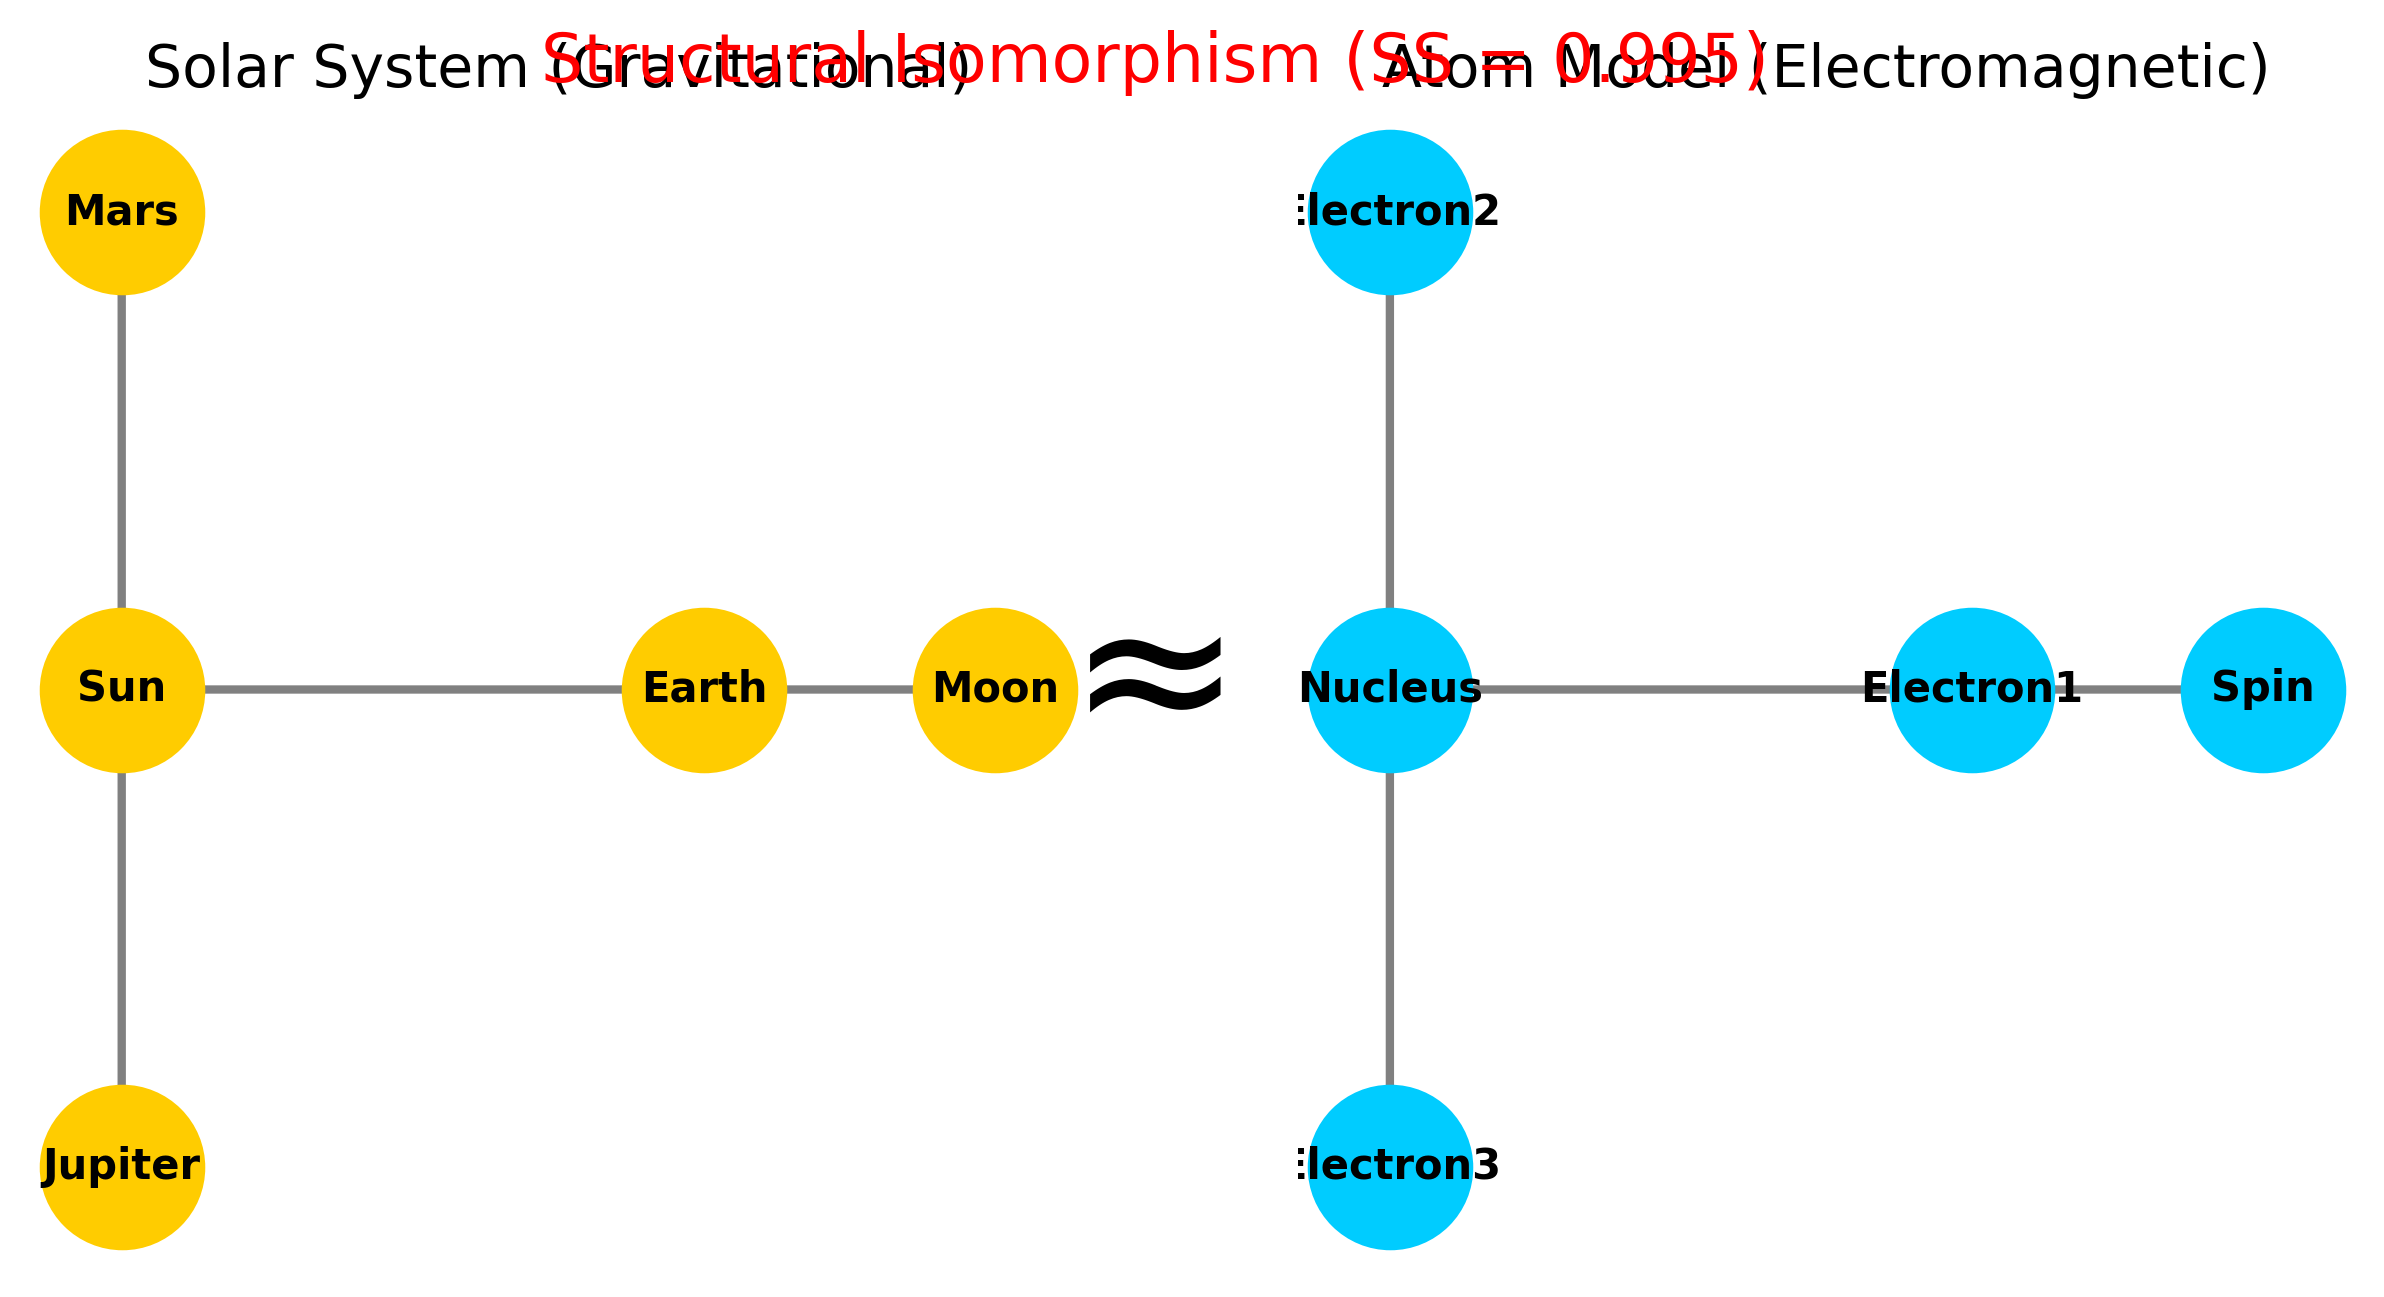
\includegraphics[width=0.9\columnwidth]{figs/analogy_isomorphism.png}
\caption{太陽系モデルと原子モデル（ボーアモデル）の構造同型性発見．異なるドメイン間でトポロジーが一致する Insight を geDIG が検出している．}
\label{fig:analogy}
\end{figure}

これは，1913年にニールス・ボーアがラザフォードの原子模型に接した際に，「太陽系と同じ構造ではないか？」と直感し（Insight），量子条件を導入してボーア・モデルを提唱した歴史的発見のプロセスを，計算論的に再現したものと言える．
認知科学者のGentnerは，類推（Analogy）の本質を「属性の類似性ではなく，関係構造の類似性（Structure-Mapping）である」と論じた\cite{gentner1983}．
geDIGは，この「関係構造の発見」を，エネルギー最小化という物理的プロセスとして自動実行できる可能性を示している．
次世代のAIは，静的なデータ学習に留まらず，このように異なる知識体系を構造レベルで架橋し，人間が見落としていた新たな科学的仮説を自律的に生成する「Scientific AI」へと進化するだろう．

%% ===========================================
%% 参考文献
%% ===========================================
\begin{thebibliography}{99}
\bibitem{friston2010} Friston, K.: The free-energy principle: a unified brain theory?, Nat. Rev. Neurosci., 11, 127--138 (2010).
\bibitem{grunwald2007} Gr\"{u}nwald, P.~D.: The Minimum Description Length Principle, MIT Press (2007).
\bibitem{vaswani2017} Vaswani, A., et al.: Attention Is All You Need, NeurIPS (2017).
\bibitem{lewis2020rag} Lewis, P., et al.: Retrieval-Augmented Generation for Knowledge-Intensive NLP Tasks, NeurIPS (2020).
\bibitem{gentner1983} Gentner, D.: Structure-mapping: A theoretical framework for analogy, Cognitive Science, 7(2), 155--170 (1983).
\bibitem{okeefe1978} O'Keefe, J., Nadel, L.: The Hippocampus as a Cognitive Map, Oxford University Press (1978).
\bibitem{tishby2000} Tishby, N., et al.: The information bottleneck method, arXiv:physics/0004057 (2000).
\bibitem{bronstein2017} Bronstein, M. M., et al.: Geometric deep learning: going beyond euclidean data, IEEE Signal Processing Magazine, 34(4), 18--42 (2017).
\bibitem{edge2024} Edge, D., et al.: From Local to Global: A Graph RAG Approach to Query-Focused Summarization, arXiv:2404.16130 (2024).
\bibitem{asai2023} Asai, A., et al.: Self-RAG: Learning to Retrieve, Generate, and Critique through Self-Reflection, arXiv:2310.11511 (2023).
\bibitem{devlin2019} Devlin, J., et al.: BERT: Pre-training of Deep Bidirectional Transformers for Language Understanding, NAACL (2019).
\bibitem{radford2019} Radford, A., et al.: Language Models are Unsupervised Multitask Learners, OpenAI Blog (2019).
\bibitem{touvron2024} Touvron, H., et al.: Llama 3: Open Foundation and Chat Models, arXiv:2407.21783 (2024).
\bibitem{bunke1997} Bunke, H.: On a relation between graph edit distance and maximum common subgraph, Pattern Recognition Letters, 18(8), 689--694 (1997).
\bibitem{riesen2009} Riesen, K., Bunke, H.: Approximate graph edit distance computation by means of bipartite graph matching, Image and Vision Computing, 27(7), 950--959 (2009).

\end{thebibliography}

\end{document}
